\documentclass[oneside,12pt,a4paper]{report}

\usepackage{AerodesignTemplate}
\selectlanguage{brazil}

% INFORMACAO DA EQUIPE
\instituicao{Universidade do Aerodesign}
\competicao{SAE BRASIL AERODESIGN 2021}
\equipe{Equipe Aerodesign}
\disciplina{Aerodinâmica}
\orientador{Santos-Dummont}

\alunos{Nome do Aluno 1 \\ Nome do Aluno 2 \\ Nome do Aluno 3 \\ Nome do Aluno 4 \\ Nome do Aluno 5 \\ Nome do Aluno 6 \\ Nome do Aluno 7 \\ Nome do Aluno 8 \\ Nome do Aluno 9 \\ Nome do Aluno 10 \\ Nome do Aluno 11 \\ Nome do Aluno 12 \\ Nome do Aluno 13 \\ Nome do Aluno 14 \\ Nome do Aluno 15 \\}

\numeroEquipe{000}
\email{aerodesign@universidade.com.br}
\logoequipe{./logos/logo_ctec_aero.png}

% INICIO DO DOCUMENTO
\begin{document}
\pagestyle{IHA-fancy-plain}
\maketitlepage

% INDEX AND LISTS
\tableofcontents

%\listoftables
%\addcontentsline{toc}{chapter}{Lista de Tabelas}

%\listoffigures
%\addcontentsline{toc}{chapter}{Lista de Figuras}

% LISTA DE SIMBOLOS
\chapter*{Lista de Símbolos}
\addcontentsline{toc}{chapter}{Lista de Símbolos}


\begin{multicols}{2}
\begin{table}[H]
    \centering
    \begin{tabular}{rl}
    $x$ & position \\
    $v$ & velocity \\
    $a$ & acceleration \\
    $t$ & time \\
    $F$ & force
\end{tabular}\\
\end{table}

\begin{table}[H]
    \centering
    \begin{tabular}{rl}
    $x$ & position \\
    $v$ & velocity \\
    $a$ & acceleration \\
    $t$ & time \\
    $F$ & force
\end{tabular}\\
\end{table}

\end{multicols} 
%\clearpage


% LISTA DE INPUTS
\chapter*{Lista de Inputs\markboth{Lista de Inputs}{}}
\addcontentsline{toc}{chapter}{Lista de Inputs}


\vspace{5cm}

\begin{figure}[H]
    \centering
    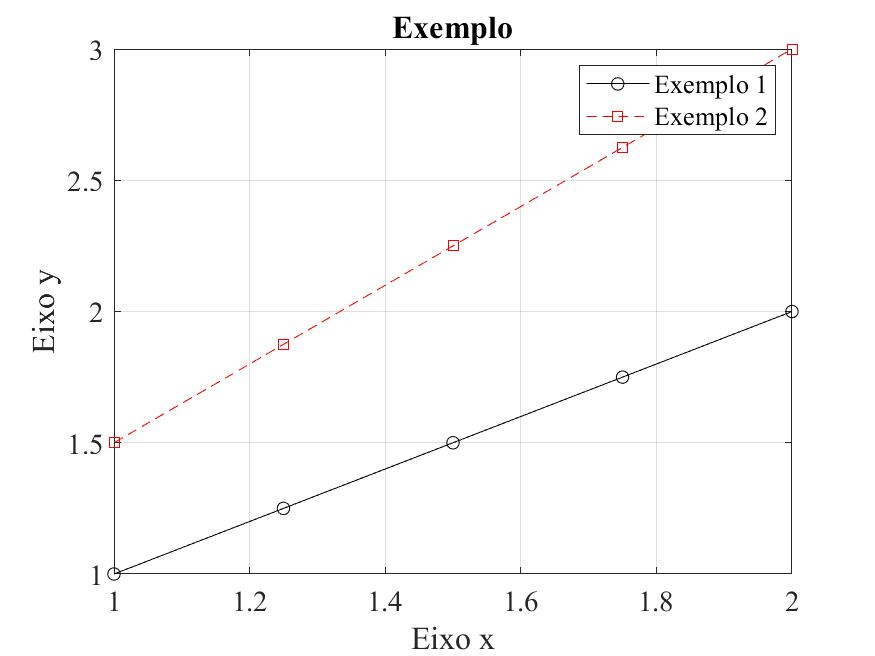
\includegraphics[width=0.8\textwidth]{images/exemplo1.jpg}
    \caption{Exemplo 1 \cite{exemploref}}
    \label{fig:exemplo111}
\end{figure}

\clearpage

\begin{figure}
    \centering
    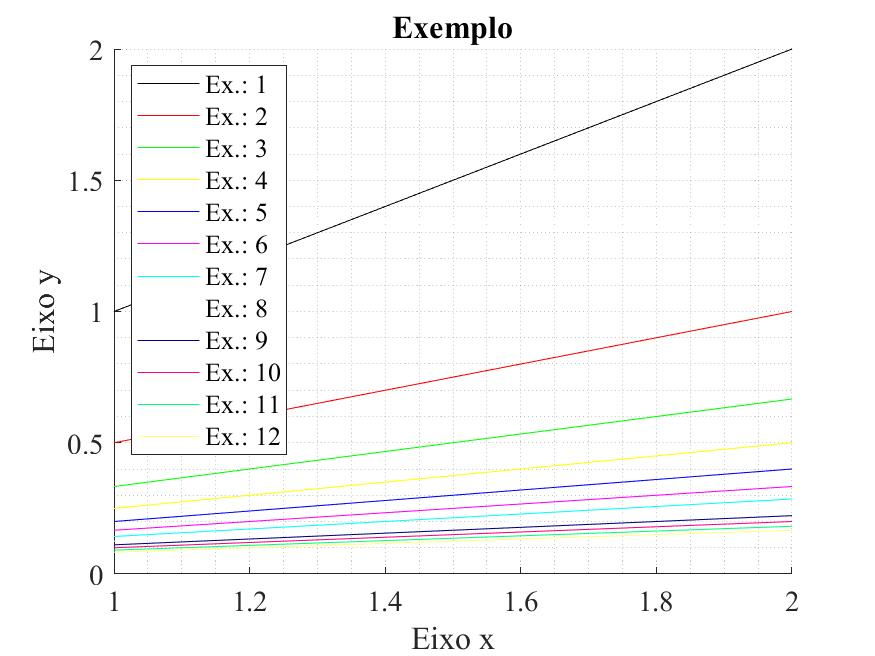
\includegraphics[width=0.8\textwidth]{images/exemplo2.jpg}
    \caption{Exemplo 2}
    \label{fig:exemplo222}
\end{figure}

\clearpage


% TEXTO TECNICO
\chapter{Introdução}
\label{cap:introducao}

\lipsum[1]

\begin{figure}[H]
    \centering
    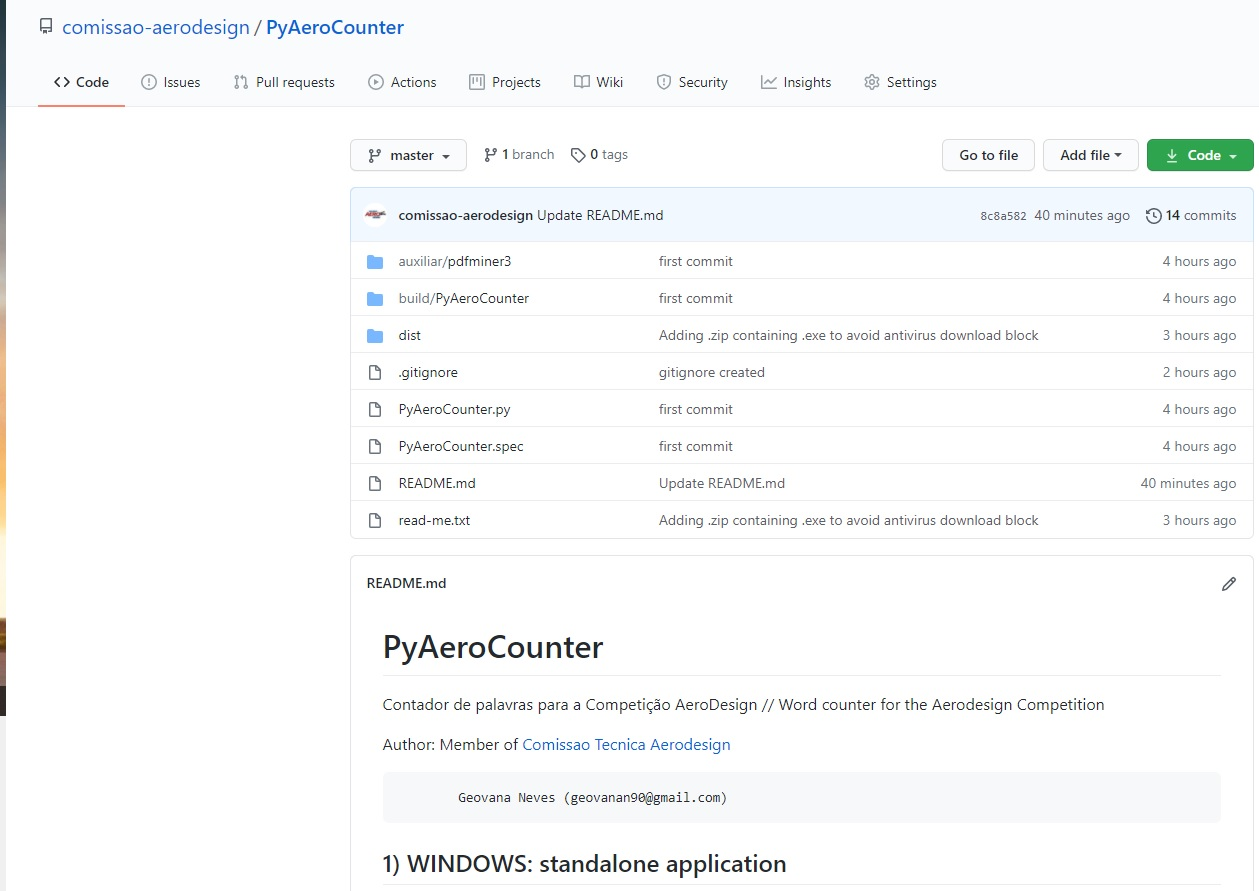
\includegraphics[width=0.8\textwidth]{images/gitfig.jpg}
    \caption{GitHub: comissao-aerodesign}
    \label{fig:my_label}
\end{figure}

\lipsum[2-4]

\section{Objetivo}

\lipsum[5]

\section{Escopo}

\lipsum[6-7]

\chapter{Conteúdo}

\lipsum[5-6]

\begin{figure}[H]
    \centering
    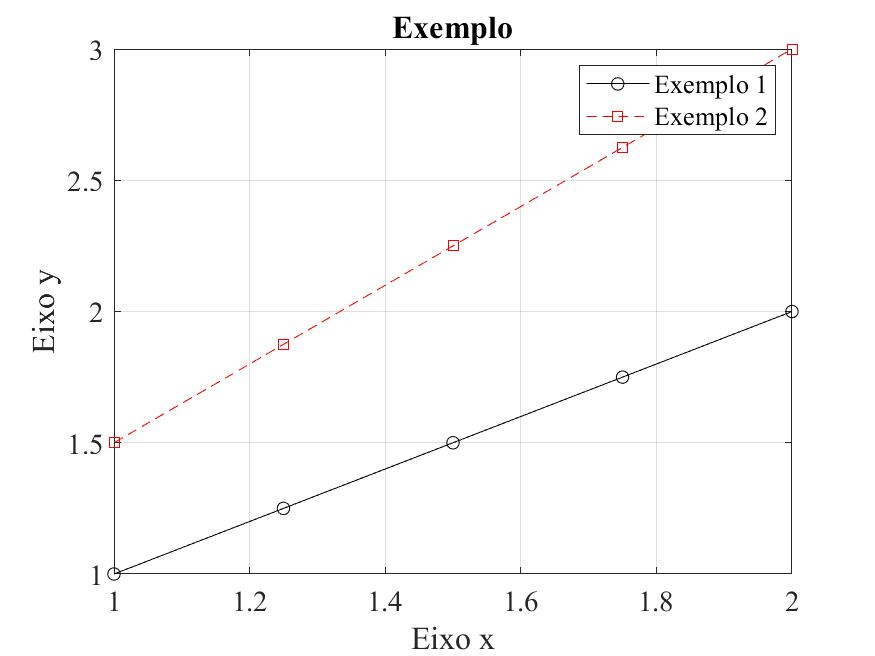
\includegraphics[width=0.8\textwidth]{images/exemplo1.jpg}
    \caption{Exemplo 1 \cite{exemploref}}
    \label{fig:exemplo 1}
\end{figure}

\lipsum[6-11]

\chapter{Conclusão}

\lipsum[11-16]

\begin{figure}[H]
    \centering
    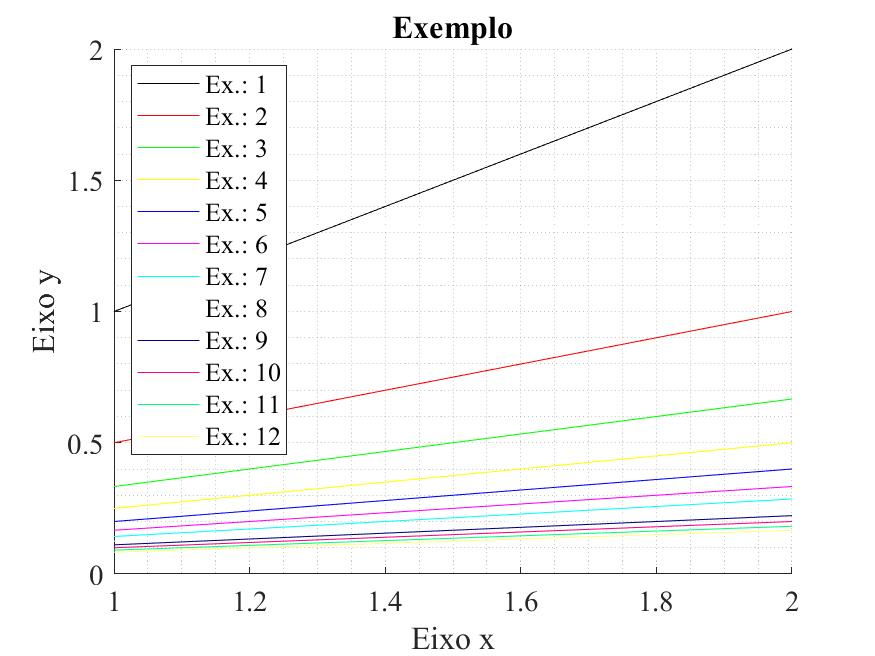
\includegraphics[width=0.8\textwidth]{images/exemplo2.jpg}
    \caption{Exemplo 2}
    \label{fig:exemplo 2}
\end{figure}

\lipsum[12-13]

% O texto tecnico pode ser divido em varios arquivos .tex para facilitar a organizacao e trabalho colaborativo
% Exemplo:
% \include{sec/introducao}
% \include{sec/teoria}
% \include{sec/metodologia}
% \include{sec/resultados}
% \include{sec/conclusao}


% LISTA DE OUTPUTS
\chapter*{Lista de Outputs\markboth{Lista de Outputs}{}}
\addcontentsline{toc}{chapter}{Lista de Outputs}


\vspace{5cm}

\begin{figure}[H]
    \centering
    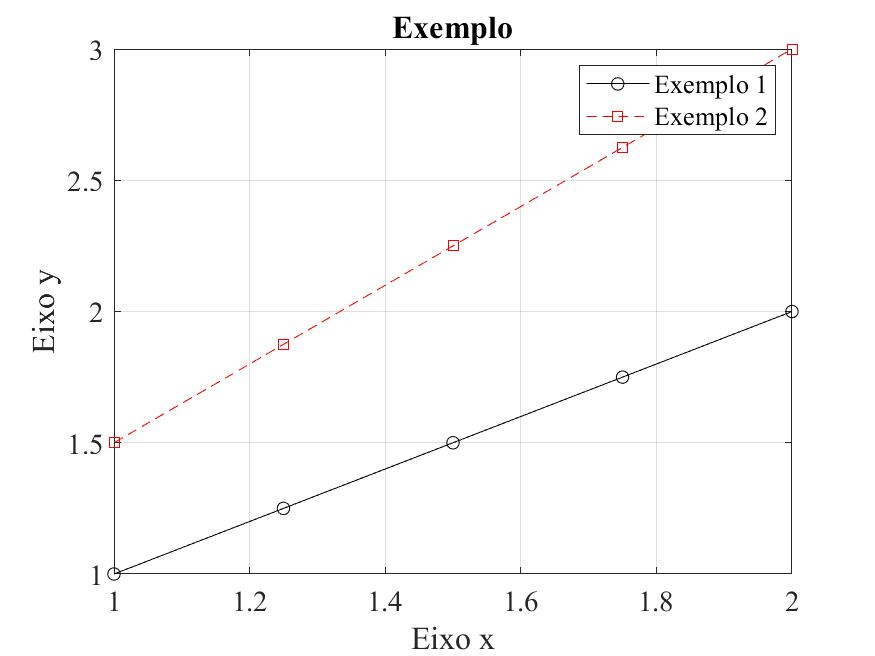
\includegraphics[width=0.8\textwidth]{images/exemplo1.jpg}
    \caption{Exemplo 1 \cite{exemploref}}
    \label{fig:exemplo11}
\end{figure}

\clearpage

\begin{figure}
    \centering
    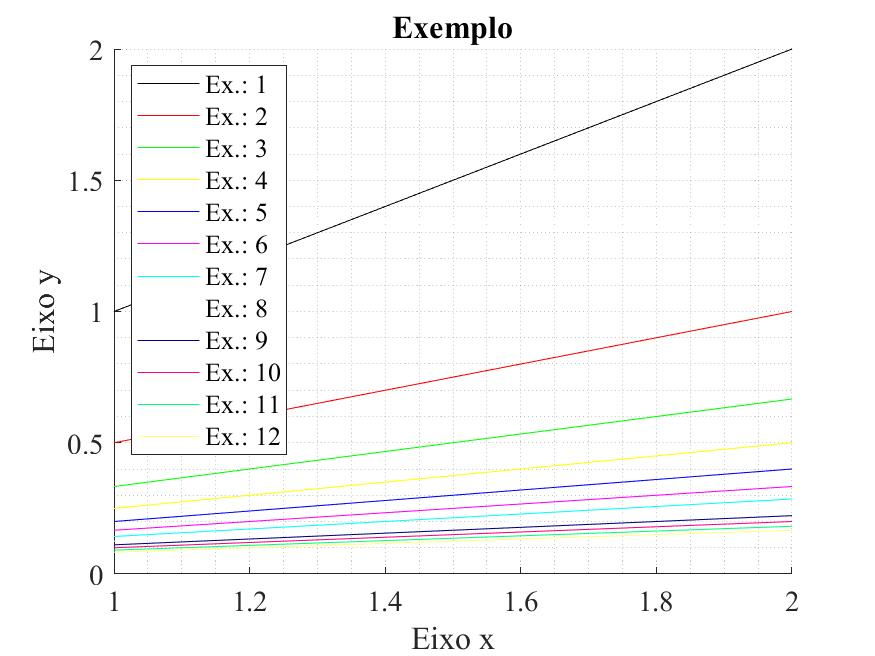
\includegraphics[width=0.8\textwidth]{images/exemplo2.jpg}
    \caption{Exemplo 2}
    \label{fig:exemplo22}
\end{figure}

\clearpage


% BIBLIOGRAFIA
\hyphenpenalty=10000 % turn off hyphenization
\bibliography{referencias}
\addcontentsline{toc}{chapter}{Referências Bibliográficas}

% APENDICE
% \appendix

\chapter{Dica para figuras em MATLAB}

\section{Script}

\small
\lstinputlisting[language=Matlab]{./scripts/exemplos_plot.m}


\section{Figuras}

\begin{figure}[H]
    \centering
    \caption{Exemplo - extensão pdf}
    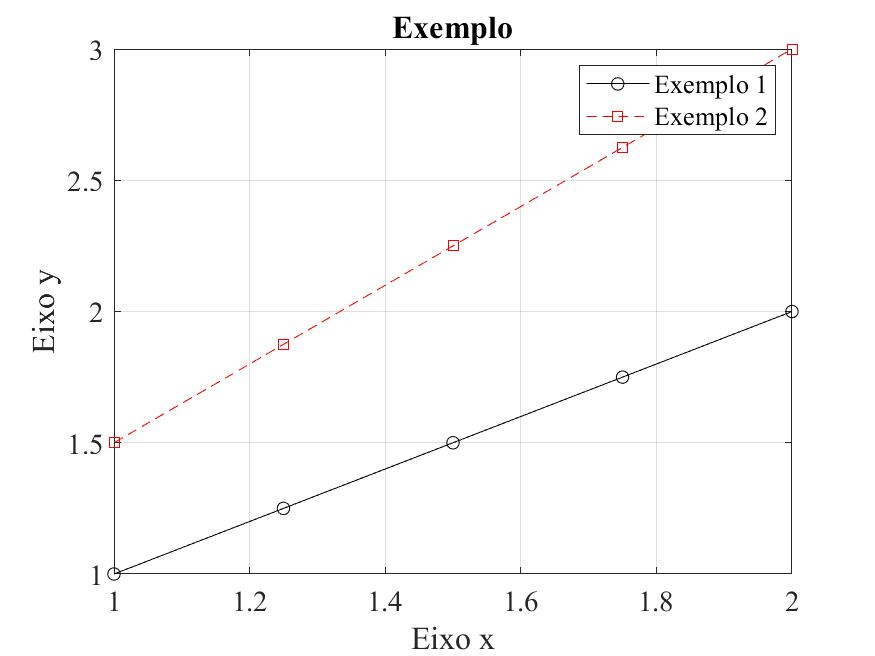
\includegraphics[trim={3.0cm 8.0cm 3.0cm 8.0cm}, clip,width=0.7\textwidth]{images/exemplo1.pdf}
\end{figure}


\begin{figure}[H]
    \centering
    \caption{Exemplo - extensão pdf}
    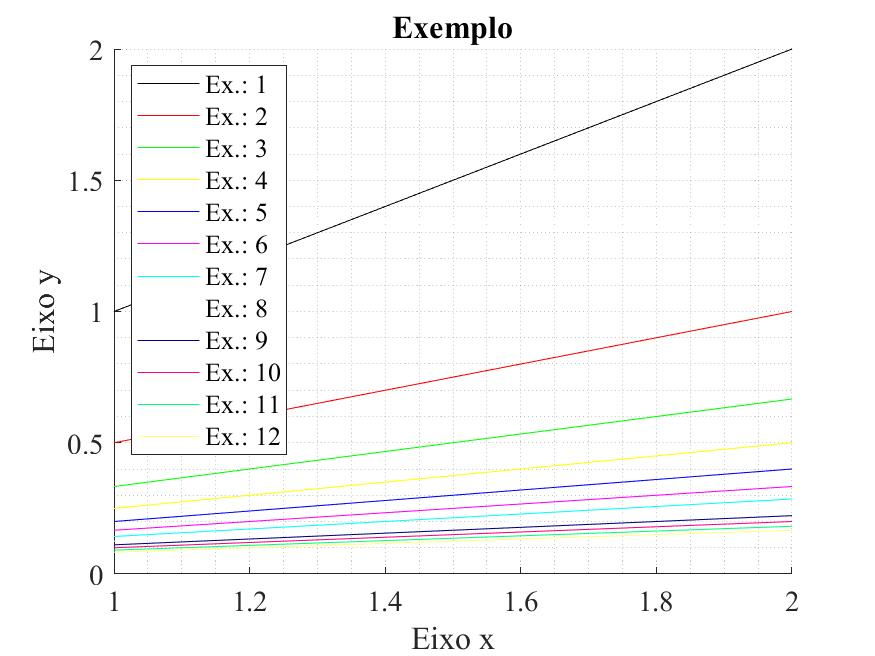
\includegraphics[trim={3.0cm 8.0cm 3.0cm 8.0cm}, clip,width=0.7\textwidth]{images/exemplo2.pdf}
\end{figure}

\begin{figure}[H]
    \centering
    \caption{Exemplo - extensão jpg}
    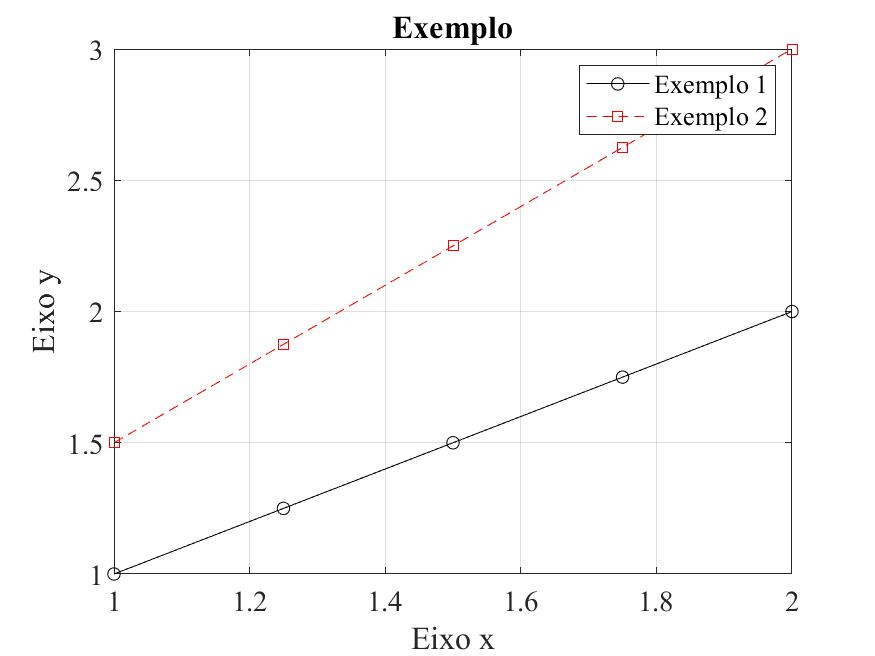
\includegraphics[width=0.7\textwidth]{images/exemplo1.jpg}
\end{figure}

\begin{figure}[H]
    \centering
    \caption{Exemplo - extensão jpg}
    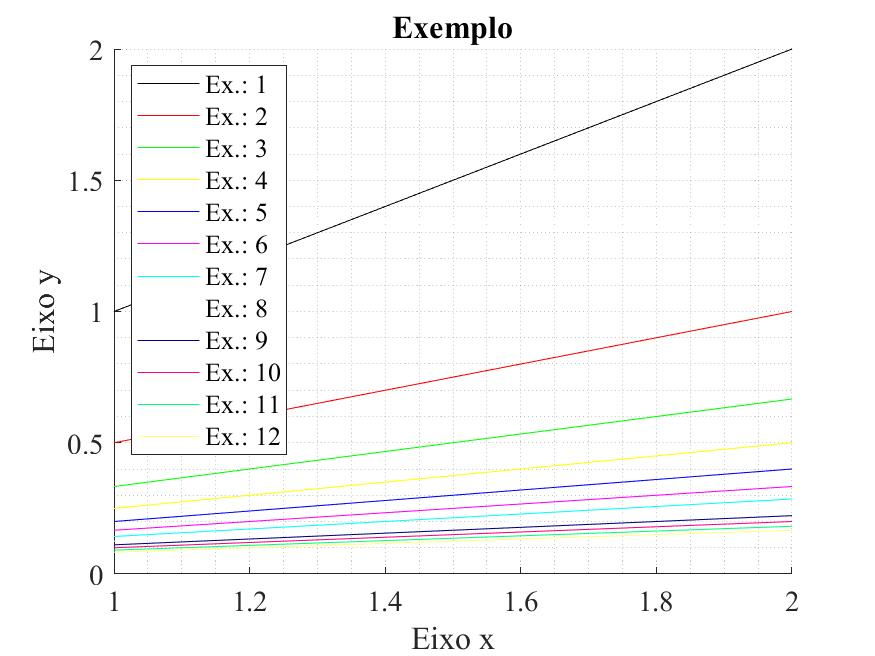
\includegraphics[width=0.7\textwidth]{images/exemplo2.jpg}
\end{figure}




\end{document}